% Created 2026-04-23 Thu 12:09
% Intended LaTeX compiler: lualatex
\DocumentMetadata{lang = en-US,pdfversion = 2.0,pdfstandard = ua-2,tagging = on,tagging-setup = {math/setup=mathml-SE},}
\documentclass[11pt]{article}
\usepackage{amsmath}
\usepackage{fontspec}
\usepackage{graphicx}
\usepackage{longtable}
\usepackage{wrapfig}
\usepackage{rotating}
\usepackage[normalem]{ulem}
\usepackage{capt-of}
\usepackage{hyperref}
\usepackage[margin=1in]{geometry}
\usepackage{fontspec}
\usepackage{verbatim, multicol, tabularx,}
\usepackage{amsmath, amsthm, amssymb, stmaryrd, latexsym, bm, listings, qtree}
\usepackage{framed}
\usepackage{xcolor,colortbl}
\usepackage{media9}
\usepackage[export]{adjustbox}
\usepackage{algorithm}
\usepackage[noend]{algpseudocode}
\usepackage{tikz,pgfplots}
\usetikzlibrary{shapes.geometric}
\let\oldquote=\quote
\let\endoldquote=\endquote
\colorlet{shadecolor}{cyan!15}
\renewenvironment{quote}{\begin{shaded*}\begin{oldquote}}{\end{oldquote}\end{shaded*}}
% From https://tex.stackexchange.com/questions/7032/good-way-to-make-textcircled-numbers
\newcommand*\circled[1]{\tikz[baseline=(char.base)]{\node[shape=circle,draw,inner sep=2pt] (char) {#1};}}
\DeclareMathOperator*{\argmin}{arg\!min}
\DeclareMathOperator*{\argmax}{arg\!max}
\lstset{frame=tb, aboveskip=1mm, belowskip=0mm, showstringspaces=false, columns=flexible, basicstyle={\scriptsize\ttfamily}, numbers=left, frame=single, breaklines=true, breakatwhitespace=true}
\hypersetup{colorlinks=true,urlcolor=blue}
\usepackage{tagpdf}
\tagpdfsetup{activate-all}
\tagpdfsetup{math/alt/use}
\usepackage{polyglossia}
\setdefaultlanguage[variant=en-US]{english}
\author{Christopher Simpkins}
\date{Kennesaw State University}
\title{Artificial Intelligence\\\medskip
\large Probabilistic Inference}
\hypersetup{
 pdfauthor={Christopher Simpkins},
 pdftitle={Artificial Intelligence},
 pdfkeywords={},
 pdfsubject={Artificial Intelligence Probabilistic Inference},
 pdfcreator={Emacs 30.2 (Org mode 9.7.11)}, 
 pdflang={English}}
\begin{document}

\maketitle
\section{Approximate Inference for Bayesian Networks}
\label{sec:org0f02931}

Exact inference in large Bayesian networks is intractable, so we need approximate inference methods.  The methods we'll learn are randomized sampling agorithms, a.k.a., \textbf{Monte Carlo} algorithms, a.k.a., \textbf{stochastic simulation}.  They work by

\begin{itemize}
\item generating random events based on the probabilities in the Bayes net and
\item counting up the different answers found in those random events.
\end{itemize}

The more the samples, the closer to the true probability distribution.


We'll learn two families of Monte carlo algorithms:

\begin{itemize}
\item direct sampling, and
\item Markov chain sampling.
\end{itemize}
\section{The Utility of Sampling}
\label{sec:org4797f06}

We observe data generated by some process.


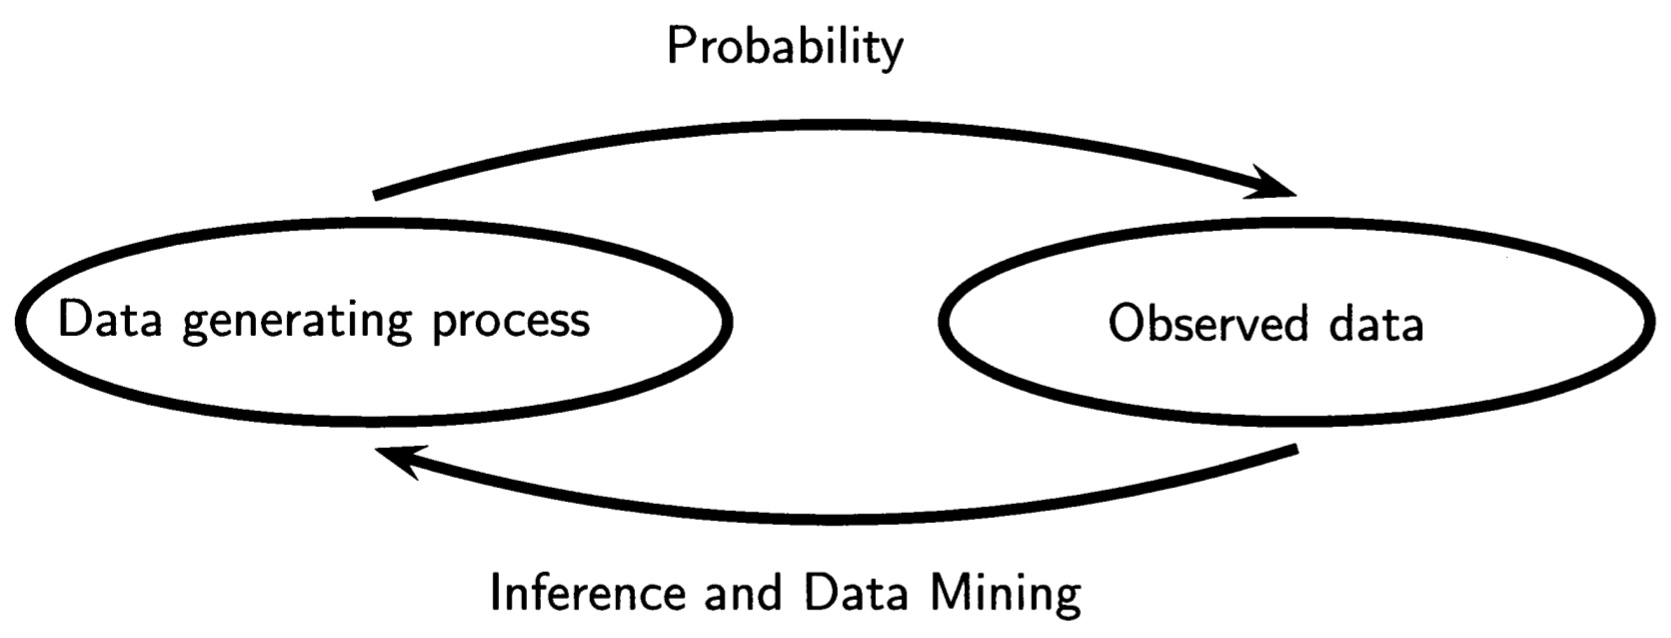
\includegraphics[alt={../../deep learning/slides/data generating process},height=2.0in]{../../deep-learning/slides/data-generating-process.jpg}


Then we use those samples to make inferences about the data generating process.

\begin{itemize}
\item In supervised machine learning we assume a distribution for the data generating process and estimate its parameters.
\item In probabilistic inference, we have a model of the full joint distribution (a Bayes net) and use it to generate samples to answer probabilistic queries.
\end{itemize}

\href{https://www.stat.cmu.edu/\~larry/all-of-statistics/}{\^{}AOS]: [All of Statistics}
\section{Computational Sampling of a Univariate Distribution}
\label{sec:orgbbaee2b}

The primitive element in any sampling algorithm is the generation of samples from a known probability distribution.




To generate samples from a single discrete or real-valued variable, \(X\),

\begin{itemize}
\item First totally order the values in the domain of \(X\).

\begin{itemize}
\item For discrete variables, if there is no natural order, just create an arbitrary ordering. Given this ordering, the cumulative probability distribution is a function of \(x\) defined by
\end{itemize}
\end{itemize}
\(f(x)=P(X \le x)\).

\begin{itemize}
\item Select a uniform random number \(y\) in the domain \([0, 1]\).
\item Let \(v\) be the value of \(X\) that maps to \(y\) in the cumulative probability distribution. That is, \(v\) is the element of \(domain(X)\) such that

\begin{itemize}
\item \(f(v) = y\) or, equivalently, \(v = f^{-1}(y)\)
\end{itemize}

\item \(X = v\) is a random sample of \(X\), chosen according to the distribution of \(X\).
\end{itemize}





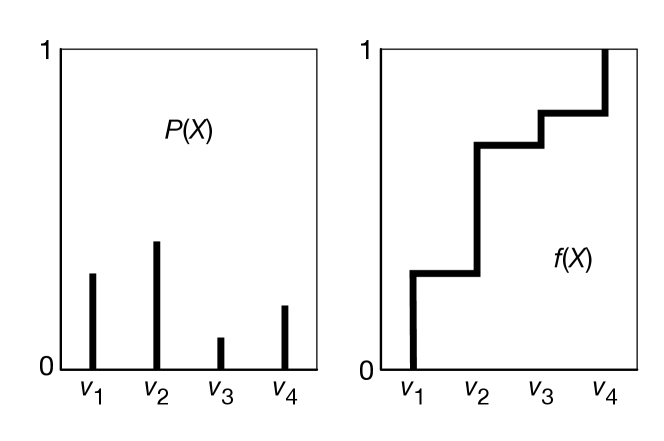
\includegraphics[height=.4\textheight]{x201.png}





This procedure works for a single variable.  If we have multiple variables and a Bayes net to represent the joint distribution over them, there are several algorithms we can use, a few of which we will see today.
\section{Prior Sampling, a.k.a., Forward Sampling}
\label{sec:org8c22cf9}

To sample from a Bayes net with no associated evidence, sample each node in topological order.

\begin{itemize}
\item Sample unconditioned nodes according to their prior distributions.

\begin{itemize}
\item Samples become fixed values for sampling CPTs of child nodes.
\end{itemize}

\item Continue sampling child nodes, in order, until all variables are sampled.
\end{itemize}


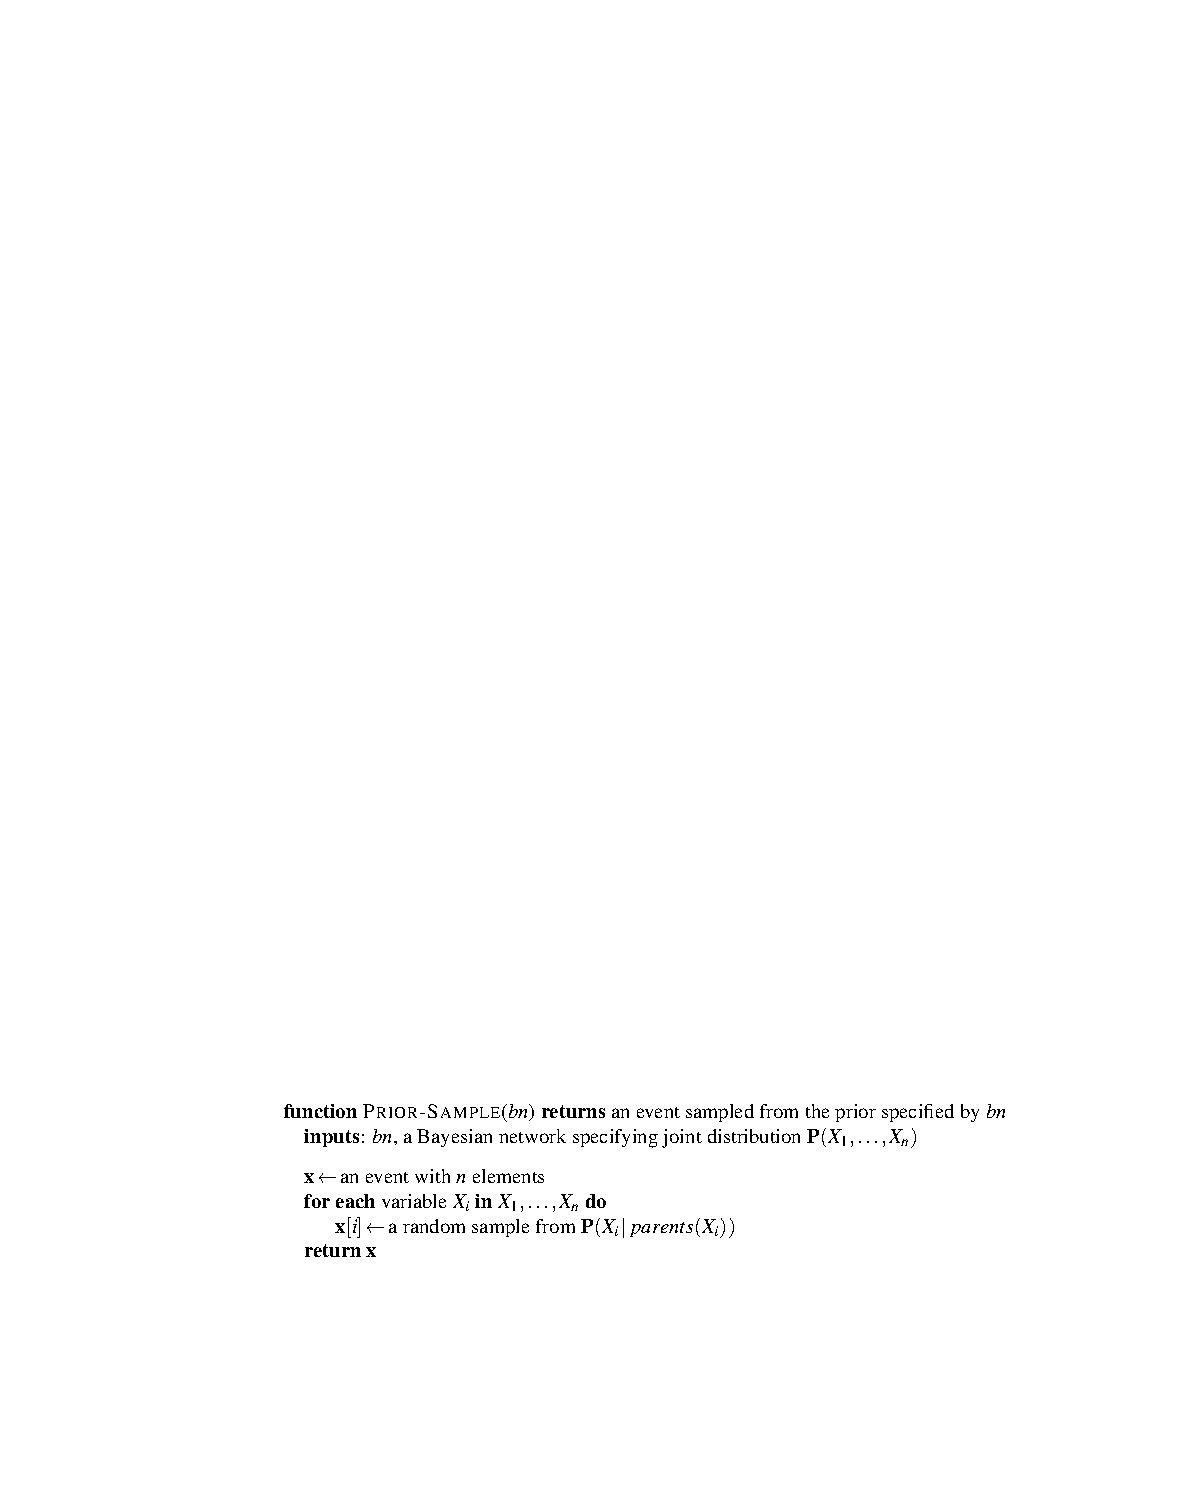
\includegraphics[alt={aima fig 13_16 bayes net prior sample algorithm},width=0.75\linewidth]{aima-fig-13_16-bayes-net-prior-sample-algorithm.pdf}
\section{Example: Generating a Sample from Sprinkler Bayes Net}
\label{sec:org26ddf4d}




\begin{enumerate}
\item Sample from \(P(Cloudy) = \langle 0.5,0.5\rangle\)

\begin{itemize}
\item Get value of true.
\end{itemize}

\item Sample from \(P(Sprinkler \mid c) = \langle 0.1,0.9 \rangle\)

\begin{itemize}
\item Get value of false.
\end{itemize}

\item Sample from \(P(Rain \mid c) = \langle 0.8,0.2 \rangle\)

\begin{itemize}
\item Get value of true.
\end{itemize}

\item Sample from \(P(WetGrass \mid \neg s, r) = \langle 0.9,0.1 \rangle\)

\begin{itemize}
\item Get value of true.
\end{itemize}
\end{enumerate}

Full sampled event: \([true, false, true, true]\)





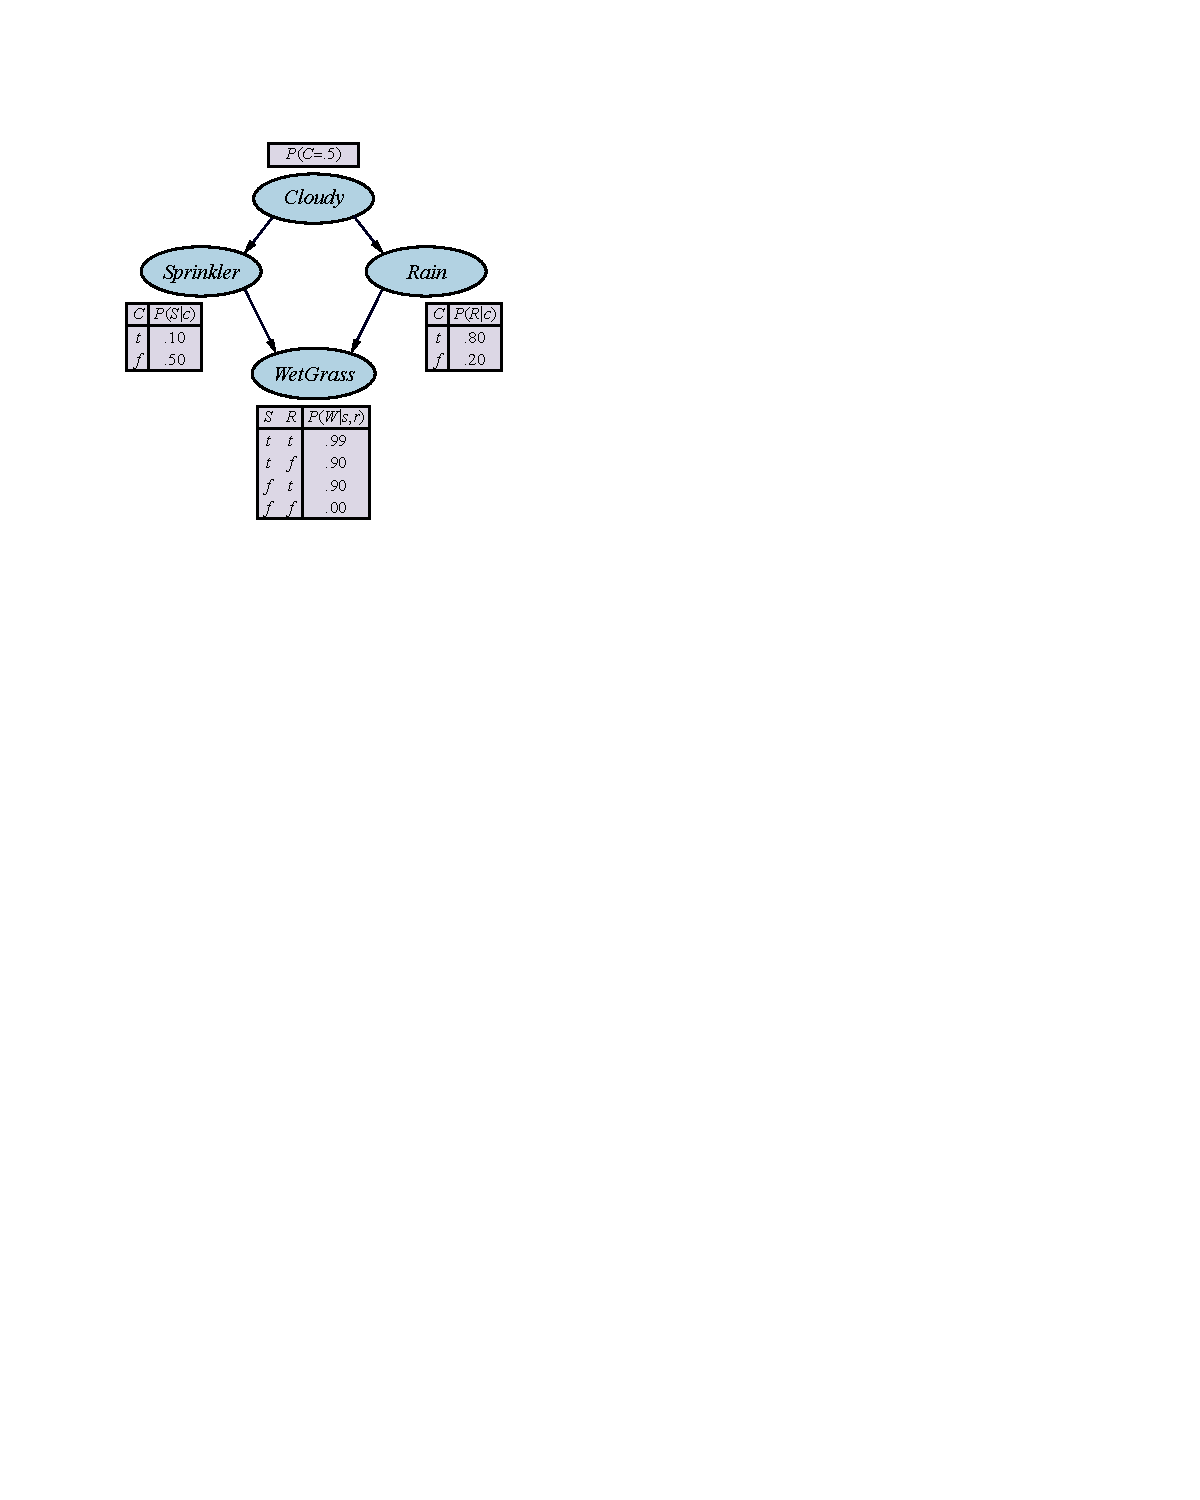
\includegraphics[alt={aima fig 13_15_a sprinkler bayes net},width=0.75\linewidth]{aima-fig-13_15_a-sprinkler-bayes-net.pdf}
\section{From Sampling to Probability Estimates}
\label{sec:orgf85335f}

A Bayes net represents a full joint distribution, so a sample generated from a Bayes net is a sample from the prior joint distribution over all the variables.  So, if \(S_{PS}\) is a sample generated by the PRIOR-SAMPLE algorithm, then:

\vspace{-.1in}
\[
S_{PS}(x_1, \dots, x_n) = \prod_{i=1}^n Pr \left( x_i \mid parents(X_i) \right) = P(x_1, \dots, x_n)
\]

To estimate these probabilities using samples, we simply generate \(N\) samples, count the number of events of interest among the \(N\) samples, and divide that number by \(N\).  This should converge to the true probability:

\vspace{-.1in}
\[
\lim_{N \to \infty} \frac{N_{PS}(x_1, \dots, x_n)}{N} = S_{PS}(x_1, \dots, x_n) = P(x_1, \dots, x_n)
\]

From the CPTs in the Bayes net, the probability of the example event we sampled, \([true, false, true, true]\) is:

\vspace{-.1in}
\[
S_{PS}(true, false, true, true) = 0.5 \cdot 0.9 \cdot 0.8 \cdot 0.9 = 0.324.
\]

So if we generated \(N = 1000\) samples, we would expect to see \([true, false, true, true]\) 324 times.
\section{Consistent Probability Estimates}
\label{sec:orgc7e872b}

An estimate that becomes exact in the large-sample limit is called \textbf{consistent}.  A consistent estimate of the probability of any partially speciified event \(x_1, \dots, x_m\) for \(x \le n\) is:

\[
P(x_1, \dots, x_m) \approx \frac{N_{PS}(x_1, \dots, x_m)}{N} = \hat{P}(x_1, \dots, x_m) \tag{13.6}
\]

That is, \(\hat{P}(x_1, \dots, x_m)\) is an approximation of \(P(x_1, \dots, x_m)\) that converges to the true probability as \(N\) approaches \(\infty\)

\begin{itemize}
\item Forward sampling generates \textbf{prior} probabilities, that is, probabilities of events prior to observing evidence.
\item What we usually want is \textbf{posterior} probabilities, \(P(X \mid \bm{e})\) -- probability of \(X\) given that we have observed evidence \(\bm{e}\).
\end{itemize}

We now turn to algorithms for computing posteriors, which use prior sampling as a subroutine.
\section{Rejection Sampling}
\label{sec:orge492e9c}

Rejection sampling is a general method for producing samples from a hard-to-sample distribution given an easy-to-sample distribution. In its simplest form, it can be used to compute conditional probabilities, that is, to determine \(P(X \mid \bm{e})\).




Let

\begin{itemize}
\item \(\hat{\bm{P}}(X \mid \bm{e})\) be a vector of the probabilities for each value of \(x \in X\) and
\item \(\bm{N}_{PS}(X, \bm{e})\) be a vector of sample counts for each \(x \in X\) where the sample is consistent with the evidence \(\bm{e}\) (the variable \textbf{C} in the algorithm).
\end{itemize}

Then:

\[
\hat{\bm{P}}(X \mid \bm{e})
= \alpha \bm{N}_{PS}(X, \bm{e})
= \frac{\bm{N}_{PS}(X, \bm{e})}{\bm{N}_{PS}(\bm{e})}
\]






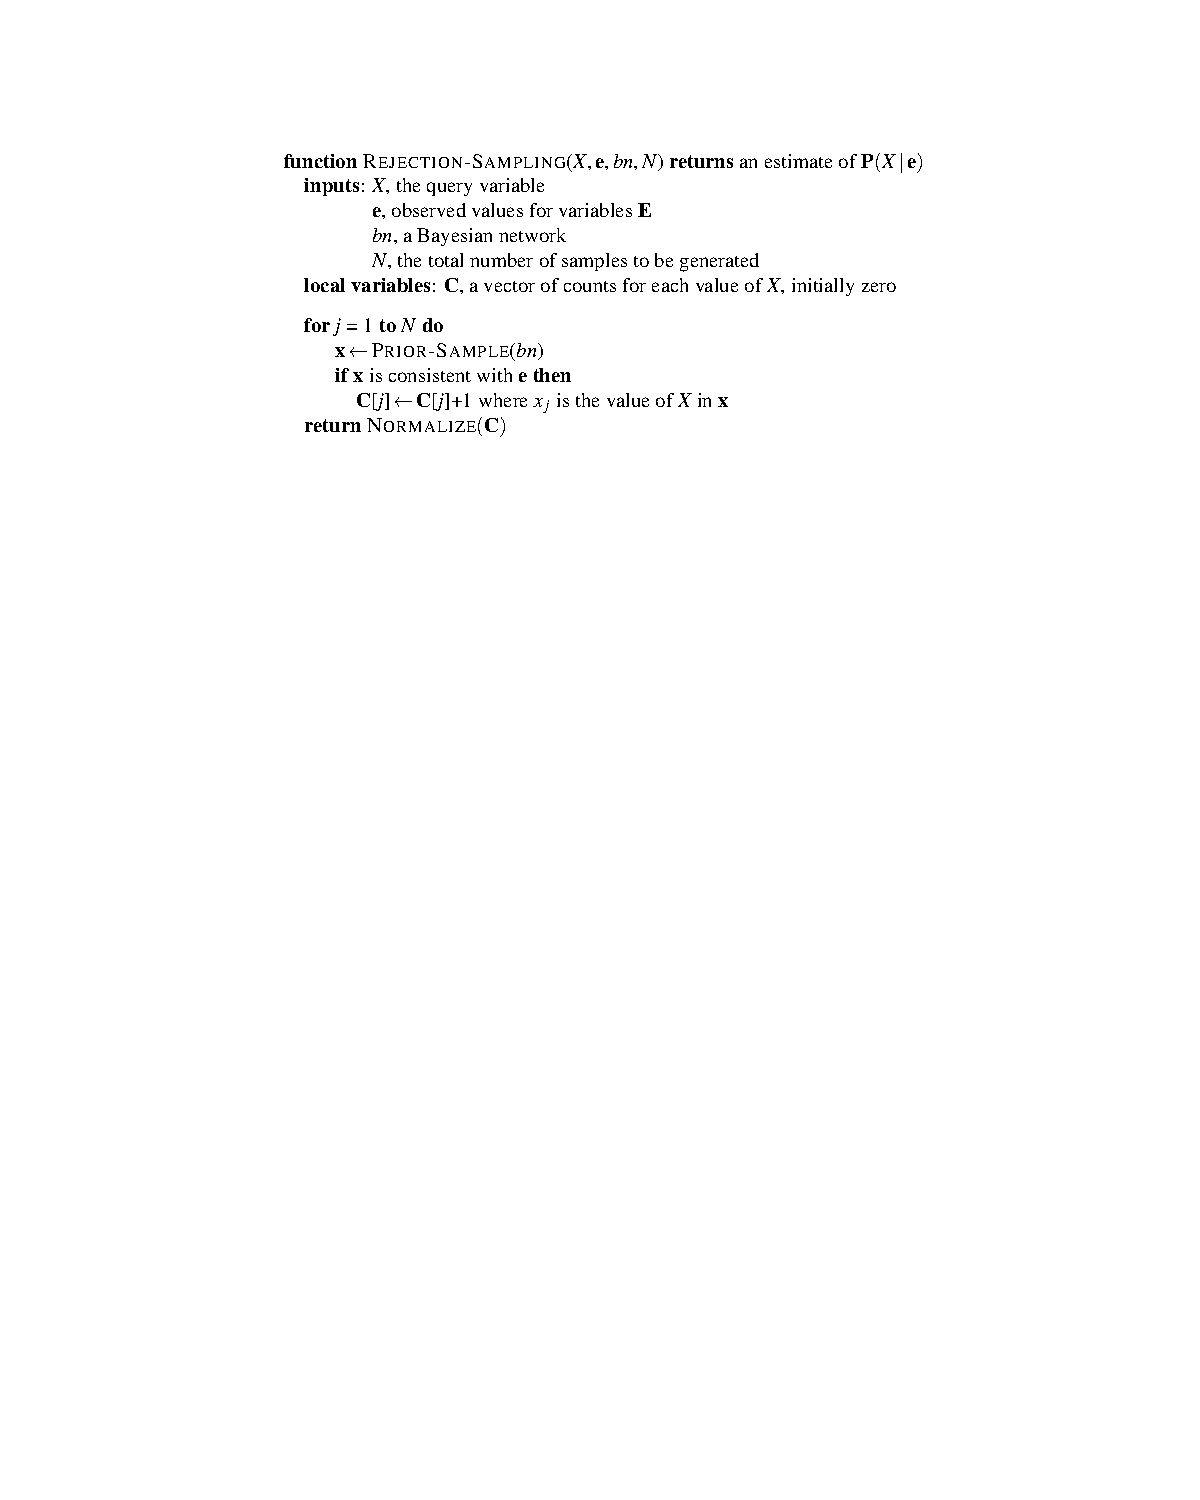
\includegraphics[alt={aima fig 13_17 bayes net rejection sampling algorithm},height=2.8in]{aima-fig-13_17-bayes-net-rejection-sampling-algorithm.pdf}
\section{Rejection Sampling Example}
\label{sec:orgf3410db}





Say we use prior sampling to generate 100 samples and we want to estimate \(\bm{P}(Rain \mid Sprinkler = true)\).

\begin{itemize}
\item 73 samples have \(Sprinkler = false\), so are \textbf{rejected}.
\item Of the 27 \textbf{accepted} samples:

\begin{itemize}
\item 8 samples have \(Rain = true\)
\item 19 samples have \(Rain = false\).
\end{itemize}
\end{itemize}

Then:

\begin{align*}
\hat{\bm{P}}(Rain \mid Sprinkler = true) &= \frac{\bm{N}_{PS}(X, \bm{e})}{\bm{N}_{PS}(\bm{e})}\\
                                         &= \frac{\langle 8, 19 \rangle}{27}\\
                                         &= \langle 0.296, 0.704 \rangle
\end{align*}

Calculating directly from the CPTs in the Bayes net would give us \(\langle 0.3, 0.7 \rangle\).





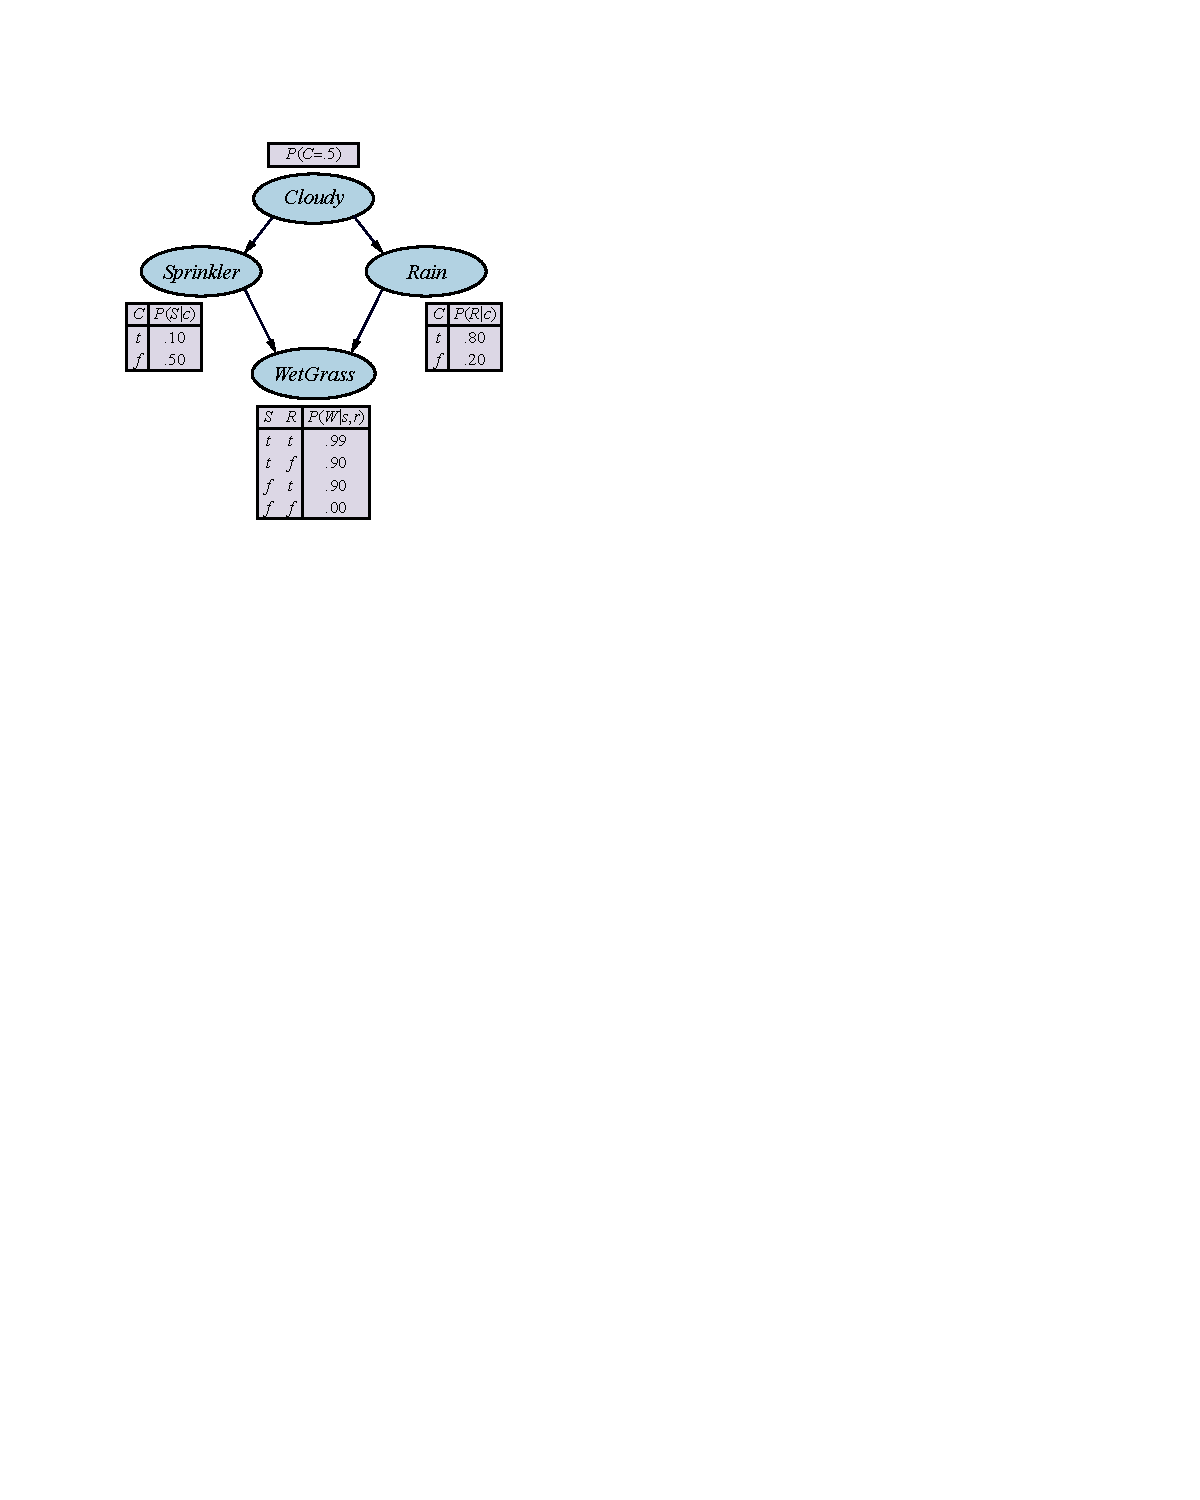
\includegraphics[alt={aima fig 13_15_a sprinkler bayes net},width=0.75\linewidth]{aima-fig-13_15_a-sprinkler-bayes-net.pdf}
\section{Importance Sampling}
\label{sec:org6527d77}

The general statistical technique of \textbf{importance sampling} aims to emulate the effect of sampling from a distribution \(P\) using samples from another distribution \(Q\), called a \textbf{proposal distribution}, whose samples are easier to obtain.

We ensure that the answers are correct in the limit by applying a correction factor \(\frac{P(\bm{x})}{Q(\bm{x})}\), also known as a \textbf{weight}, to each sample \(\bm{x}\) when counting up the samples.

Our query variable will always be one of the nonevidence variables, \(Z\).  The idea of importance sampling is to sample from \(P(\bm{z} \mid \bm{e})\):

\vspace{-.1in}
\[
\hat{P} (\bm{z} \mid \bm{e}) = \frac{ N_P (\bm{z}) }{ N } \approx P(\bm{z} \mid \bm{e})
\]

but using an arbitrary distribution \(Q(\bm{z})\):

\[
\hat{P} (\bm{z} \mid \bm{e}) =
\frac{ N_Q (\bm{z}) }{ N } \frac{ P(\bm{z} \mid \bm{e}) }{ Q(\bm{z}) }  \approx
Q(\bm{z}) \frac{ P(\bm{z} \mid \bm{e}) }{ Q(\bm{z}) } =
P(\bm{z} \mid \bm{e})
\]

The question is: which \(Q\) to use?  We want \(Q\) as close as possible to \(P(\bm{z} \mid \bm{e})\) with \(Q(\bm{z}) \ne 0\) whenever \(P(\bm{z} \mid \bm{e}) \ne 0\).  The most common approach is \textbf{likelihood weighting} \ldots{}
\section{Likelihood Weighting}
\label{sec:org944645b}

Fix the values for the evidence variables \(\bm{E}\) and sample all the nonevidence variables in topological order, each conditioned on its parents -- guarantees each sample consistent with evidence.

Let the sampling distribution be \(Q_{WS}\) and nonevidence variables be \(\bm{Z} = \{ Z_1, \dots, Z_l \}\). Then:

\vspace{-.2in}
\[
Q_{WS}(\bm{z}) = \prod_{i = 1}^l P(z_i \mid parents(Z_i))
\]

Now we need to know the weight for each sample.  By general scheme for importance sampling:

\vspace{-.1in}
\[
w(\bm{z}) = \frac{ P(\bm{z}\mid \bm{e}) }{ Q_{WS}(\bm{z}) } = \alpha \frac{ P(\bm{z},\bm{e}) }{ Q_{WS}(\bm{z}) }
\]

where the normalizing factor \(\alpha = \frac{1}{P(e)}\) is the same for all samples.  Since \(\bm{z}\) and \(\bm{e}\) cover all the variables in the Bayes net, \(P(\bm{z}, \bm{e})\) is the product of the conditional probabilities for the nonevidence variables times the product of the conditional probabilities for the evidence variables:

\vspace{-.2in}
\begin{align*}
w(\bm{z}) &= \alpha \frac{ P(\bm{z},\bm{e}) }{ Q_{WS}(\bm{z}) }
          = \alpha \frac{ \prod_{i = 1}^l P(z_i \mid parents(Z_i)) \prod_{i = 1}^m P(e_i \mid parents(E_i))  }
          { \prod_{i = 1}^l P(z_i \mid parents(Z_i))  }\\
          &= \alpha \prod_{i = 1}^m P(e_i \mid parents(E_i)) \tag{14.9}
\end{align*}

The name of this method comes from the fact that probabilities of evidence are generally called likelihoods.
\section{Likelihood Weighting Algorithm}
\label{sec:org9dd9b39}


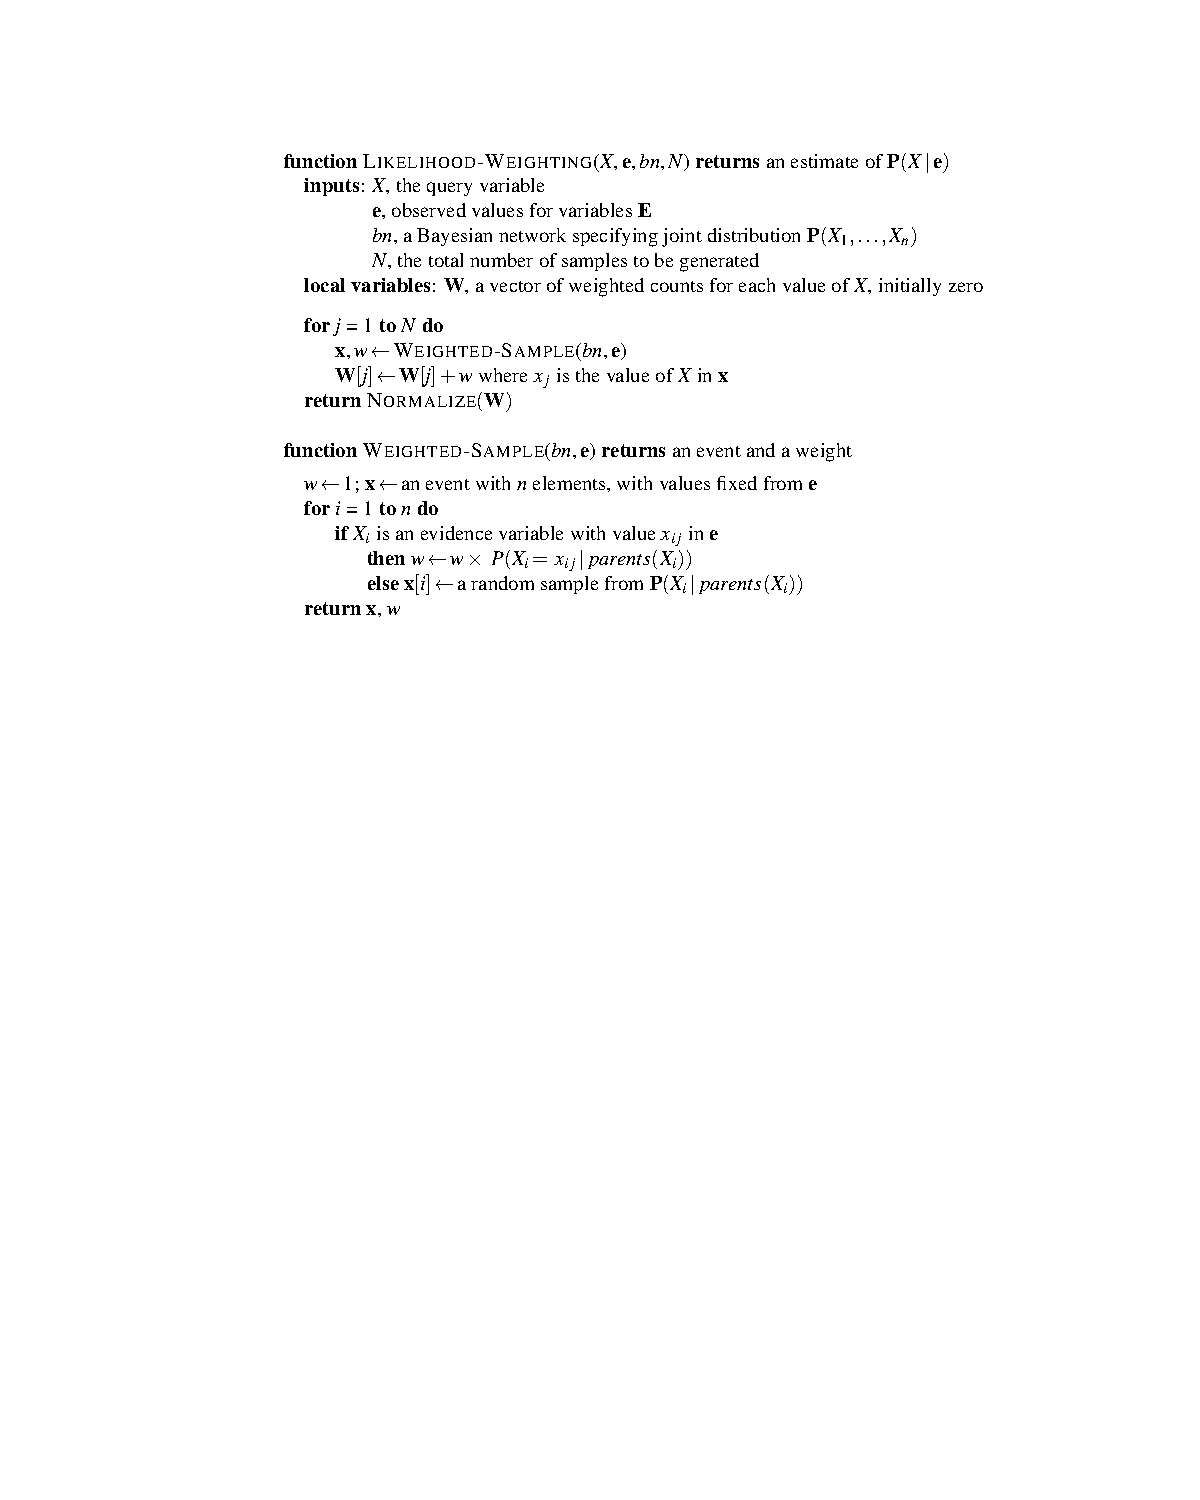
\includegraphics[alt={aima fig 13_18 bayes net likelihood weighting algorithm},width=0.75\linewidth]{aima-fig-13_18-bayes-net-likelihood-weighting-algorithm.pdf}
\section{Likelihood Weighting Example}
\label{sec:org33563aa}




Given the query

\begin{itemize}
\item \(P(Rain \mid Cloudy= true, WetGrass= true)\)
\end{itemize}

and the ordering

\begin{itemize}
\item \(Cloudy, Sprinkler, Rain, WetGrass\),
\end{itemize}

we initialize \(w = 1.0\) and proceed as follows:

\begin{enumerate}
\item \(Cloudy\) is an evidence variable with value true. Therefore, we set

```\{=latex\}
\vspace{-.1in}
\[
    w \gets w \cdot P(c) = 0.5.
    \]
```
\end{enumerate}


\begin{enumerate}
\item \(Sprinkler\) is not an evidence variable, so sample from \$P(Sprinkler \mid Cloudy= true) =
\end{enumerate}
\(\langle\) 0.1,0.9 \(\rangle\)\$; suppose this returns false.

\begin{enumerate}
\item \(Rain\) is not an evidence variable, so sample from \(P(Rain \mid Cloudy = true) = \langle 0.8,0.2 \rangle\); suppose this returns true.

\item \(WetGrass\) is an evidence variable with value true. Therefore, we set

```\{\texttt{latex\}
    \textbackslash{}vspace\{-.2in\}
    \textbackslash{}[
    w \textbackslash{}gets w \textbackslash{}times P(WetGrass=true \textbackslash{}mid \textbackslash{}neg s, r) = 0.5 \textbackslash{}cdot 0.9} 0.45.
$\backslash$]
```
\end{enumerate}

Here WEIGHTED-SAMPLE returns the event \([true,false,true,true]\) with weight 0.45, which we tally under \(Rain = true\).





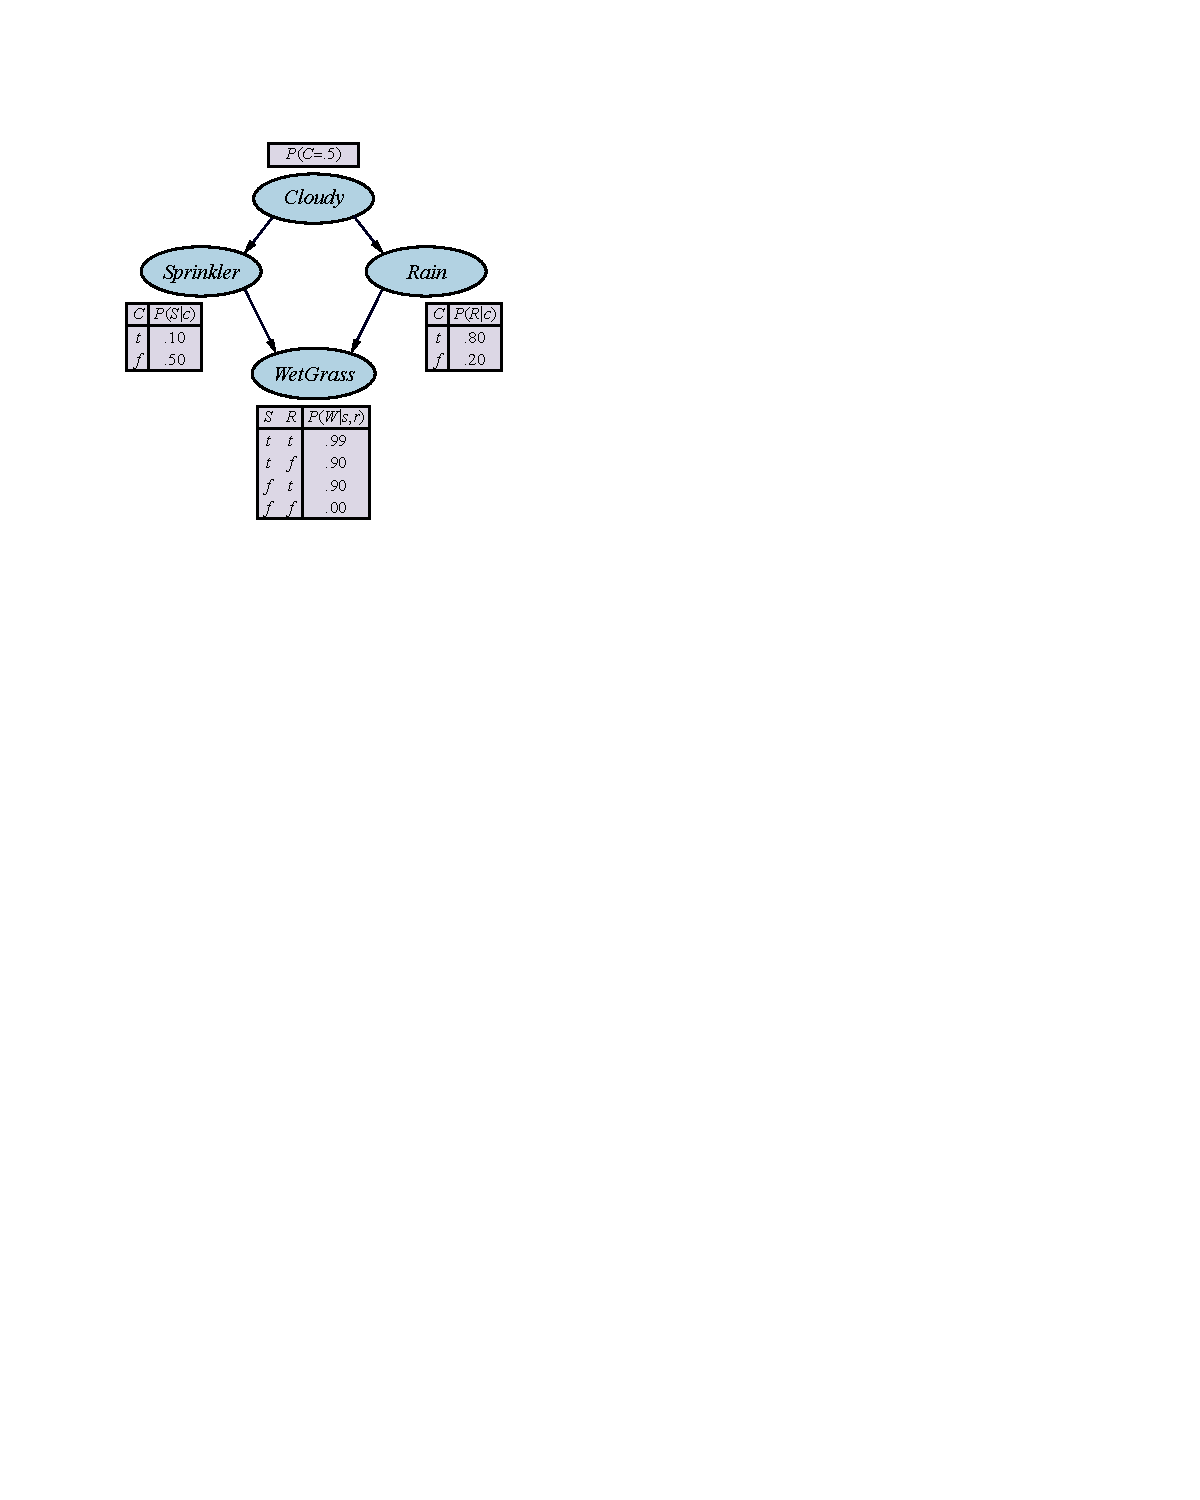
\includegraphics[alt={aima fig 13_15_a sprinkler bayes net},width=0.75\linewidth]{aima-fig-13_15_a-sprinkler-bayes-net.pdf}
\section{Rejection vs. Importance Sampling}
\label{sec:orgcf30717}


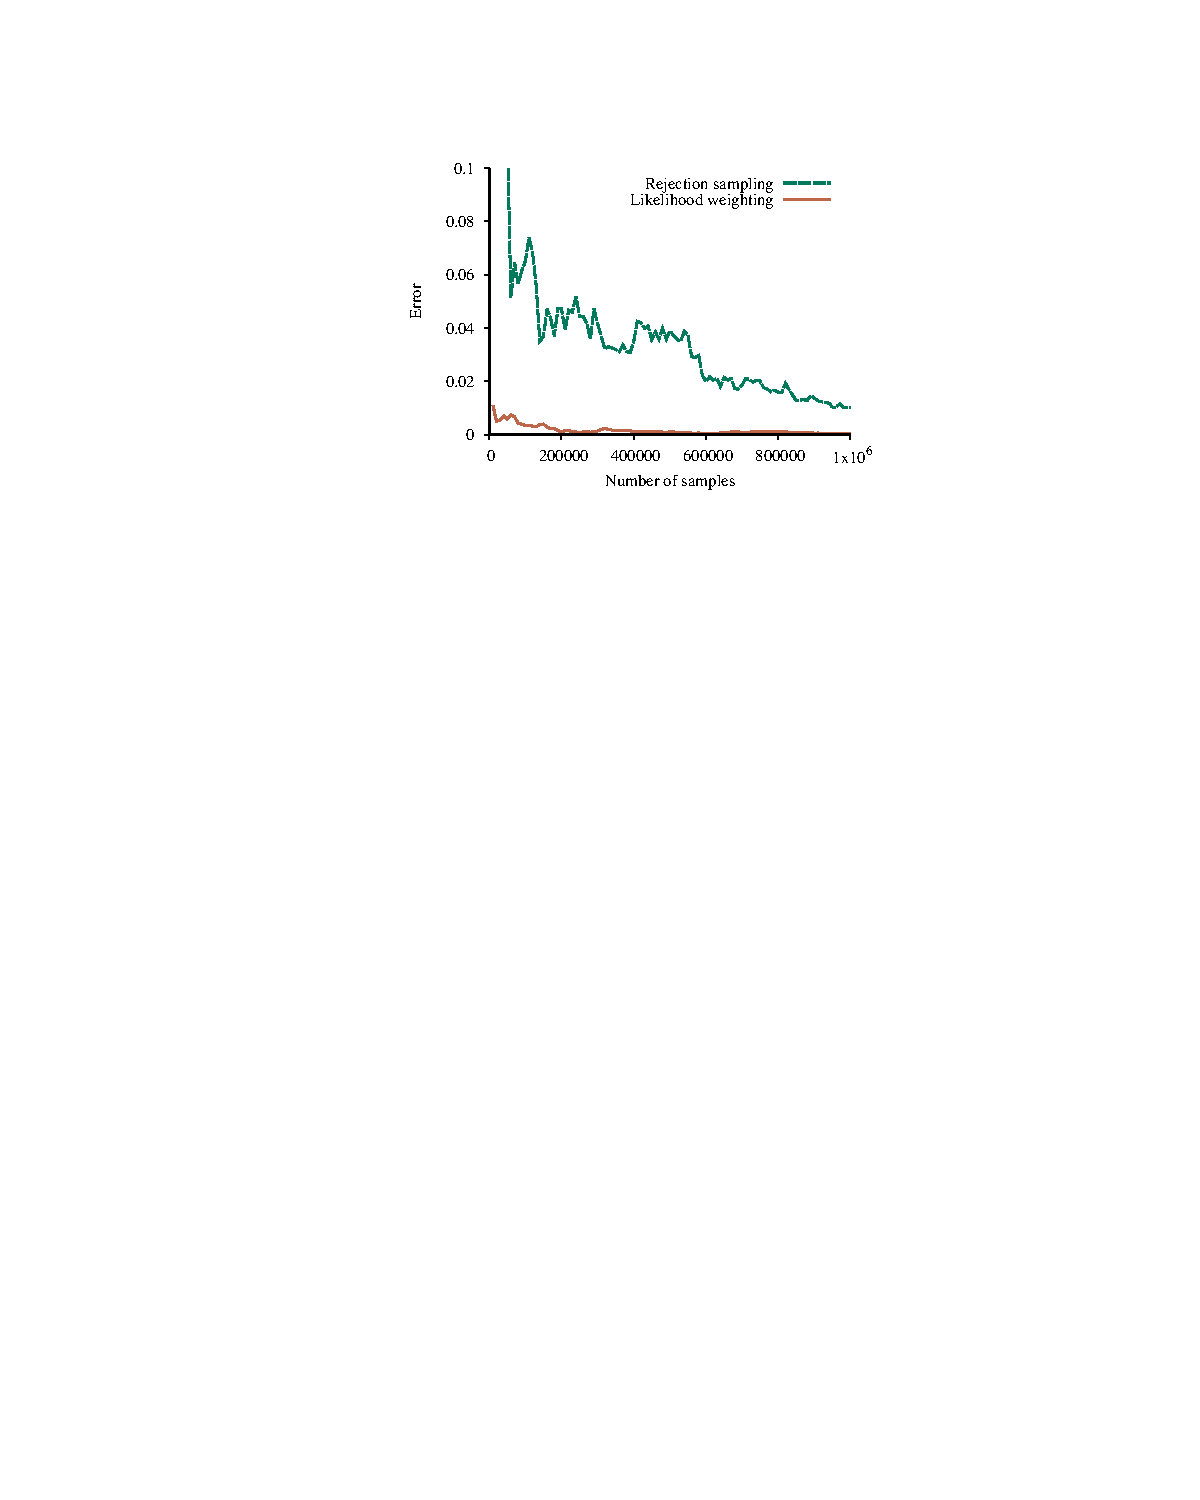
\includegraphics[alt={aima fig 13_19 performance plot rejection sampling likelihood weighting},width=0.75\linewidth]{aima-fig-13_19-performance-plot-rejection-sampling-likelihood-weighting.pdf}
\section{Markov Chain Monte Carlo (MCMC) Algorithms}
\label{sec:orgdcb476c}

Instead of generating each sample from scratch, MCMC algorithms generate a sample by making a random change to the preceding sample.

Think of an MCMC algorithm as being in a particular current state that specifies a value for every variable and generating a next state by making random changes to the current state.

We'll learn two MCMC algorithms:

\begin{itemize}
\item Gibbs sampling, and
\item Metropolis-Hastings
\end{itemize}
\section{Gibbs Sampling and Markov Blankets}
\label{sec:org860618d}



\includegraphics[alt={bee gees blanket},height=3.2in]{bee-gees-blanket.jpg}
\section{Conditional Independence Relations}
\label{sec:org6771567}


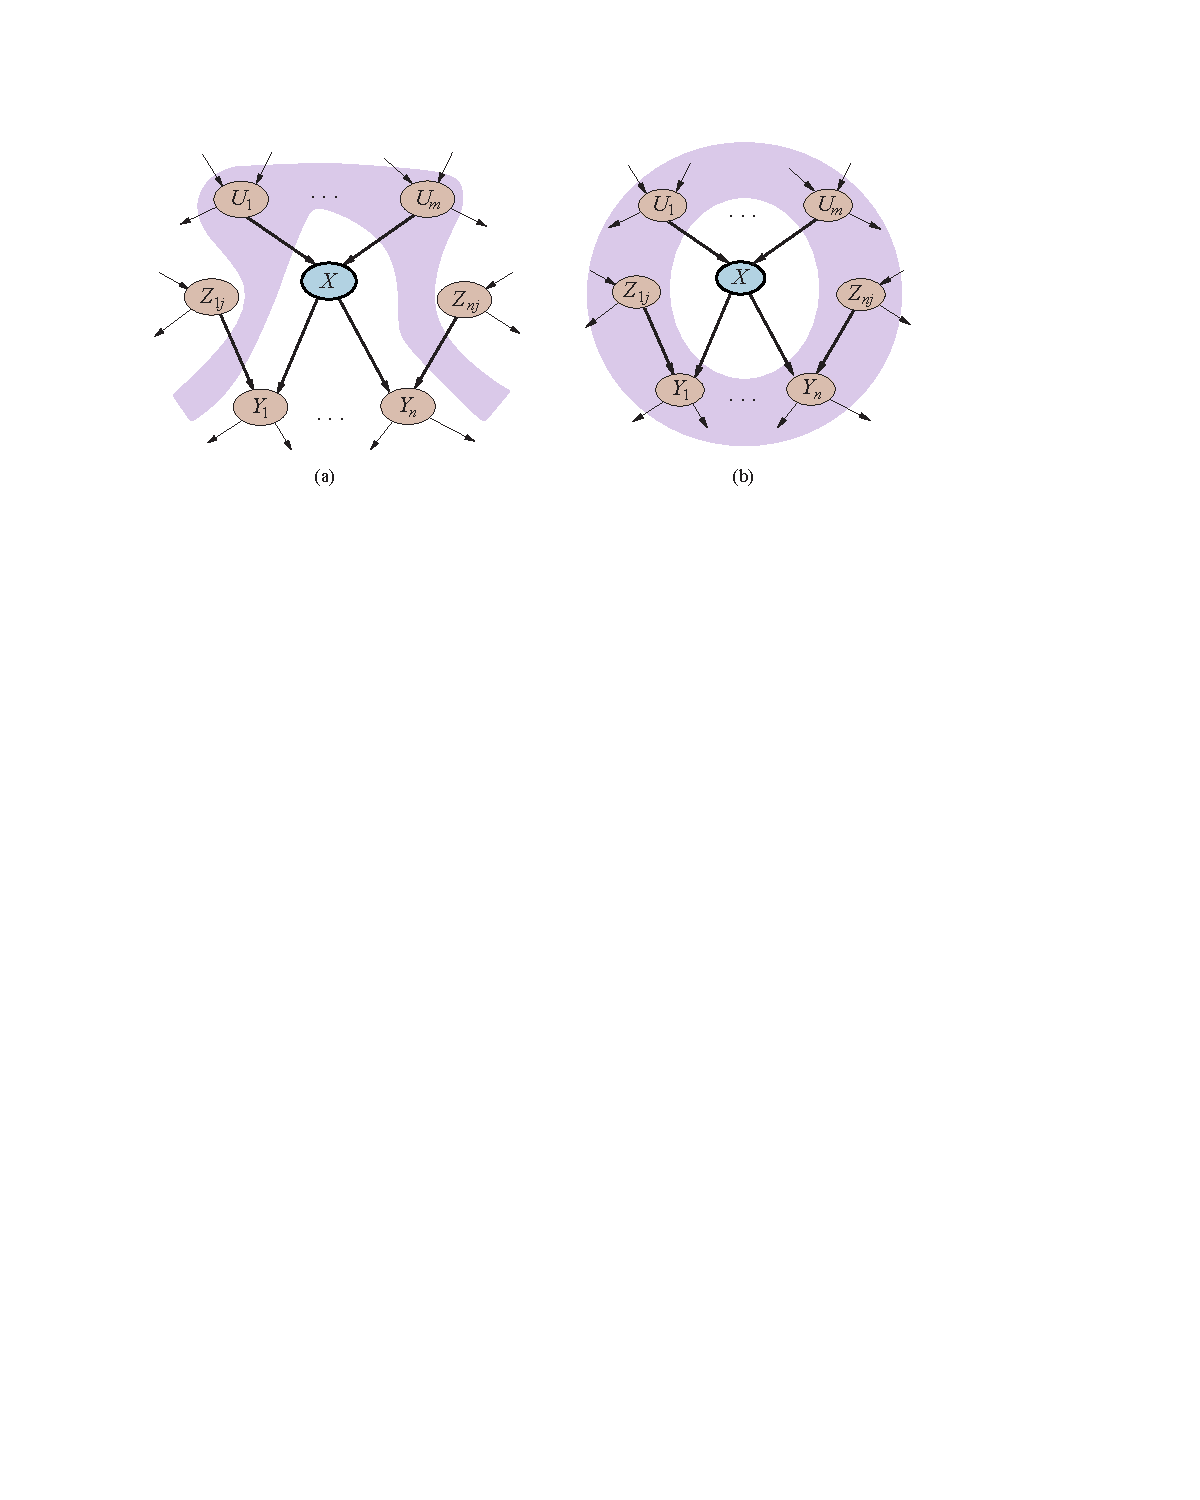
\includegraphics[alt={aima fig 13_04 markov blankets},height=1.4in]{aima-fig-13_04-markov-blankets.pdf}


\begin{itemize}
\item (a) Each variable is conditionally independent of its non-descendants, given its parents.

\item (b) A variable is conditionally independent of all other nodes in the network, given its parents, children, and children's parents -- that is, given its \textbf{Markov blanket}.
\end{itemize}

For example, the variable \(Burglary\) is independent of \(JohnCalls\) and \(MaryCalls\), given \(Alarm\) and \(Earthquake\).
\section{Gibbs Sampling}
\label{sec:orgff77235}




\begin{itemize}
\item Fix the evidence variables.
\item Start in a arbitrary state sampled from the nonevidence variables.

\begin{itemize}
\item Each \(X_i\) is sampled from the values in its Markov blanket, \(mb(X_i)\)
\end{itemize}

```\{=latex\}
\[
    P(x_i \mid mb(X_i)) = \alpha P(x_i \mid parents(X_i)) \prod_{Y_j \in Children(X_i)} P(y_i \mid parents(Y_j)) \tag{13.10}
    \]
\vspace{.1in}
```

\item Wander the state space randomly, keeping the evidence variables fixed and flipping one nonevidence variable by sampling from a distribution calculated Equation 13.10.
\end{itemize}





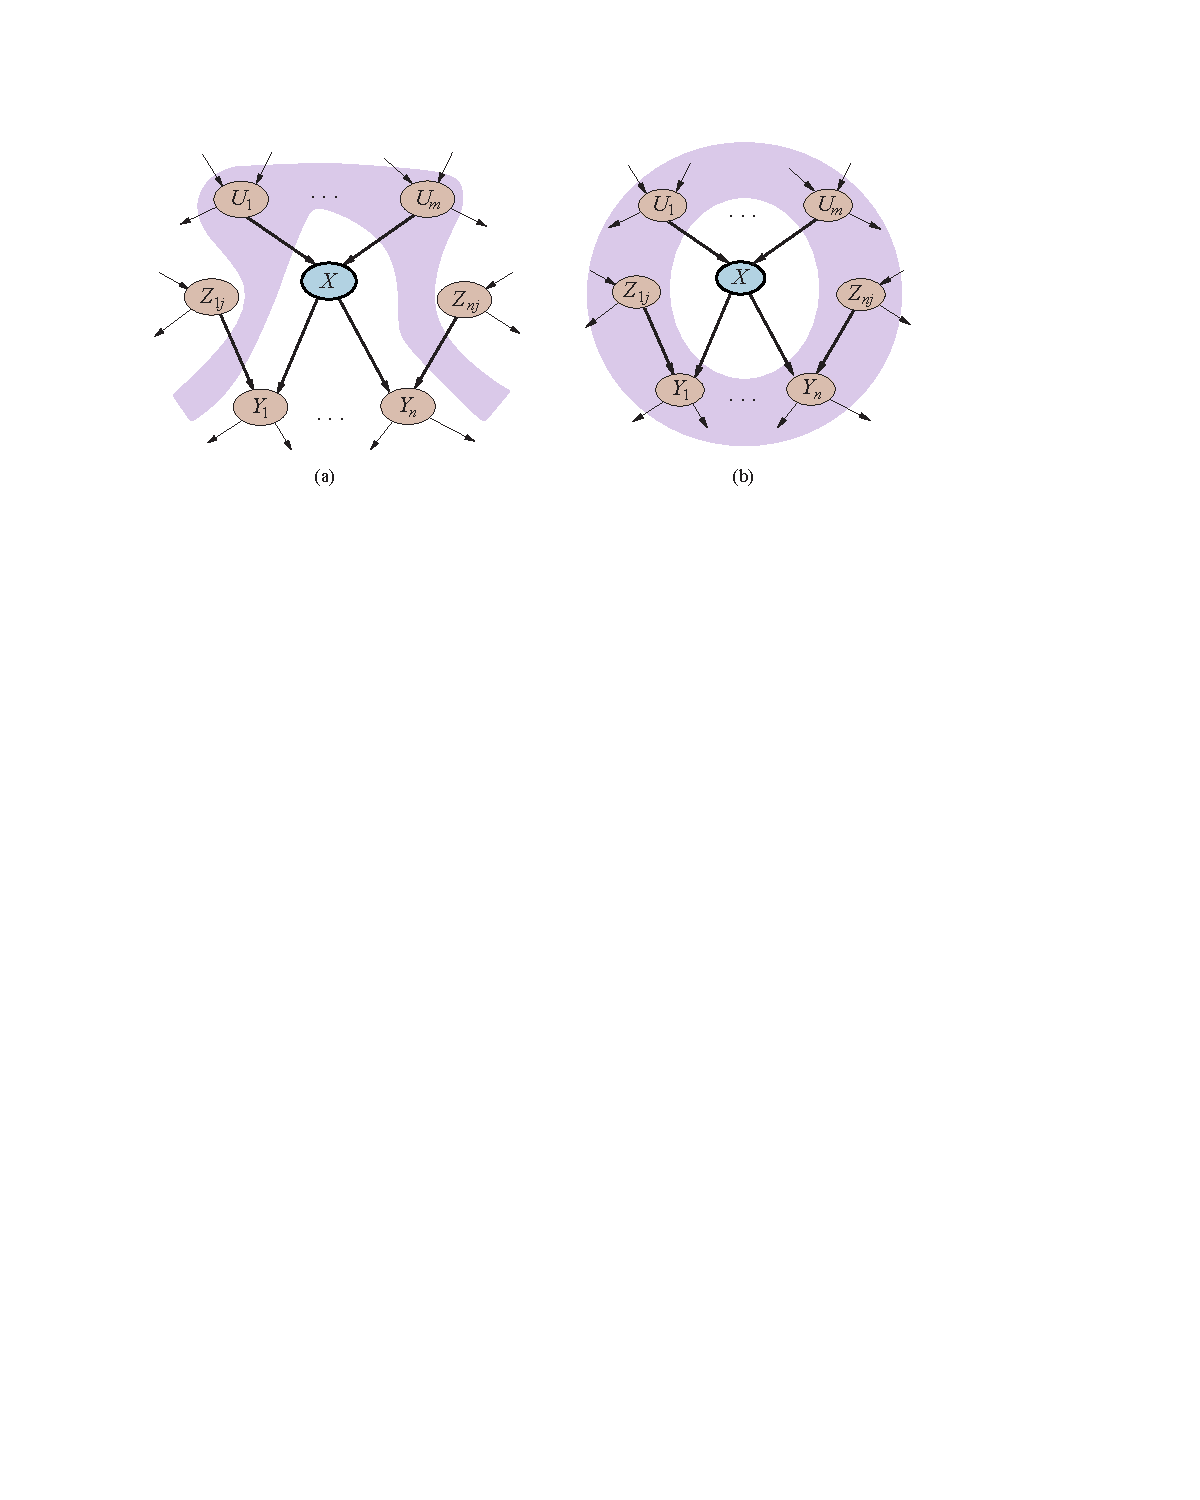
\includegraphics[alt={aima fig 13_04 markov blankets},height=3.2in]{aima-fig-13_04-markov-blankets.pdf}





Gibbs sampling for \(X_i\) means sampling conditioned on the current values of the variables in its Markov blanket.
\section{Gibbs Sampling Example: Step 1}
\label{sec:orgd3bc3f7}




Consider the query \(P(Rain \mid Sprinkler = true,WetGrass= true)\).

\begin{itemize}
\item Evidence variables \(Sprinkler\) and \(WetGrass\) fixed to observed values (true), nonevidence variables \(Cloudy\) and \(Rain\)  initialized randomly to, say, true and false respectively.

\begin{itemize}
\item Initial state is \([true, \textbf{true}, false, \textbf{true}]\). Fixed evidence variables marked in bold.
\end{itemize}
\end{itemize}

Now the nonevidence variables \(Z_i\) are sampled repeatedly in some random order according to a probability distribution \(\rho(i)\) for choosing variables. For example:






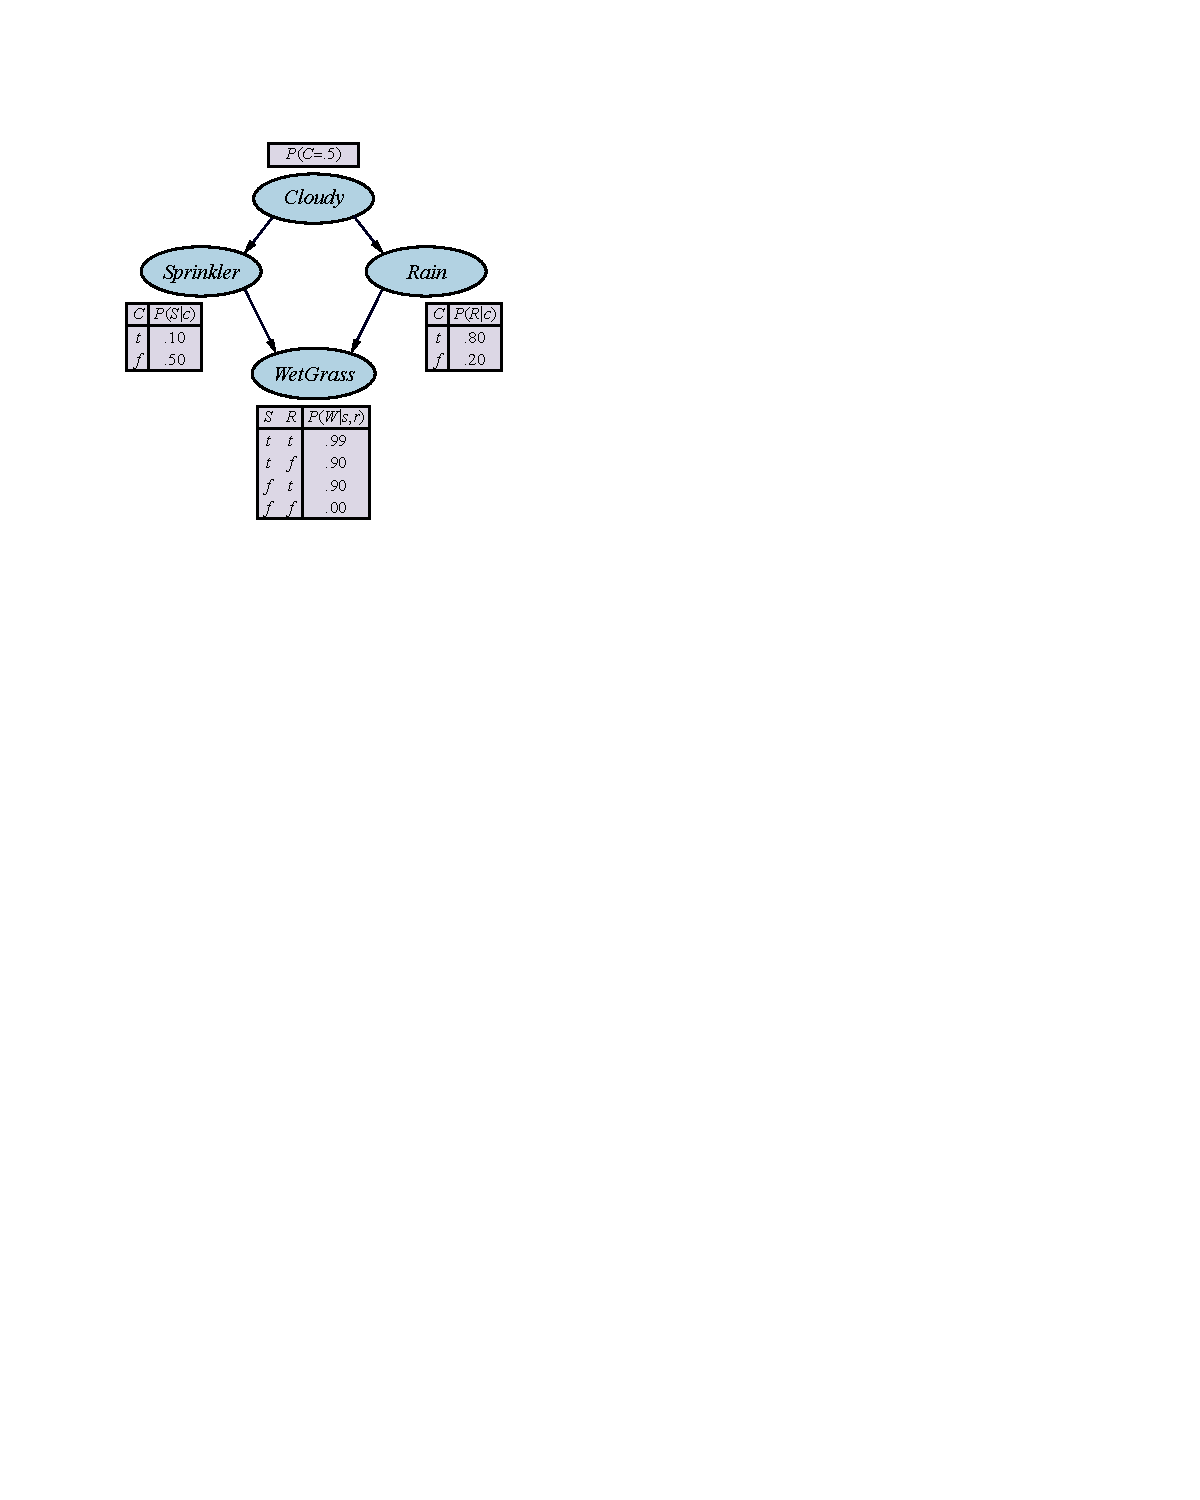
\includegraphics[alt={aima fig 13_15_a sprinkler bayes net},height=1.2in]{aima-fig-13_15_a-sprinkler-bayes-net.pdf}






\begin{enumerate}
\item \(Cloudy\) is chosen and then sampled, given the current values of its Markov blanket: in this case, we sample from \(P(Cloudy|Sprinkler= true,Rain= false)\) whose distribution is calculated using Equation 13.10:
\end{enumerate}

\vspace{-.2in}
\begin{align*}
P(x_i \mid mb(X_i))      &= \alpha P(x_i \mid parents(X_i)) \prod_{Y_j \in Children(X_i)} P(y_i \mid parents(Y_j)) \tag{13.10}\\
P(c \mid s, \neg r)      &= \alpha P(c) P(s \mid c) P(\neg r \mid c) = \alpha 0.5 \cdot 0.1 \cdot 0.2\\
P(\neg c \mid s, \neg r) &= \alpha P(\neg c) P(s \mid \neg c) P(\neg r \mid \neg c) = \alpha 0.5 \cdot 0.5 \cdot 0.8
\end{align*}

yielding \(\alpha \langle 0.001, 0.020 \rangle \approx \langle 0.048, 0.952 \rangle\)

\begin{itemize}
\item Suppose the result is \(Cloudy= false\). Then the new current state is \([false, \textbf{true}, false, \textbf{true}]\).
\end{itemize}
\section{Gibbs Sampling Example: Step 2}
\label{sec:orgd23d469}




\begin{enumerate}
\item Sampling \(\rho(i)\) then chooses \(Rain\) as next variable.  We sample from \(P(Rain \mid Cloudy= false,Sprinkler= true,WetGrass= true)\) using Equation 13.10 (just like Step 1, not shown here).

\item Suppose this yields \(Rain= true\). The new current state is \([false, \textbf{true}, true, \textbf{true}]\).
\end{enumerate}

Figure on the right shows the complete Markov chain for the case where variables are chosen
uniformly, i.e., \(\rho (Cloudy) = \rho (Rain) = 0.5\).

\begin{itemize}
\item The algorithm wanders around in this graph, following links with stated probabilities.
\item Each state visited during this process is a sample that contributes to the estimate for the query variable Rain. - If the process visits 20 states where Rain is true and 60 states where Rain is false, then the answer to the query is \(NORMALIZE(\langle 20,60 \rangle) = \langle 0.25,0.75 \rangle\).
\end{itemize}





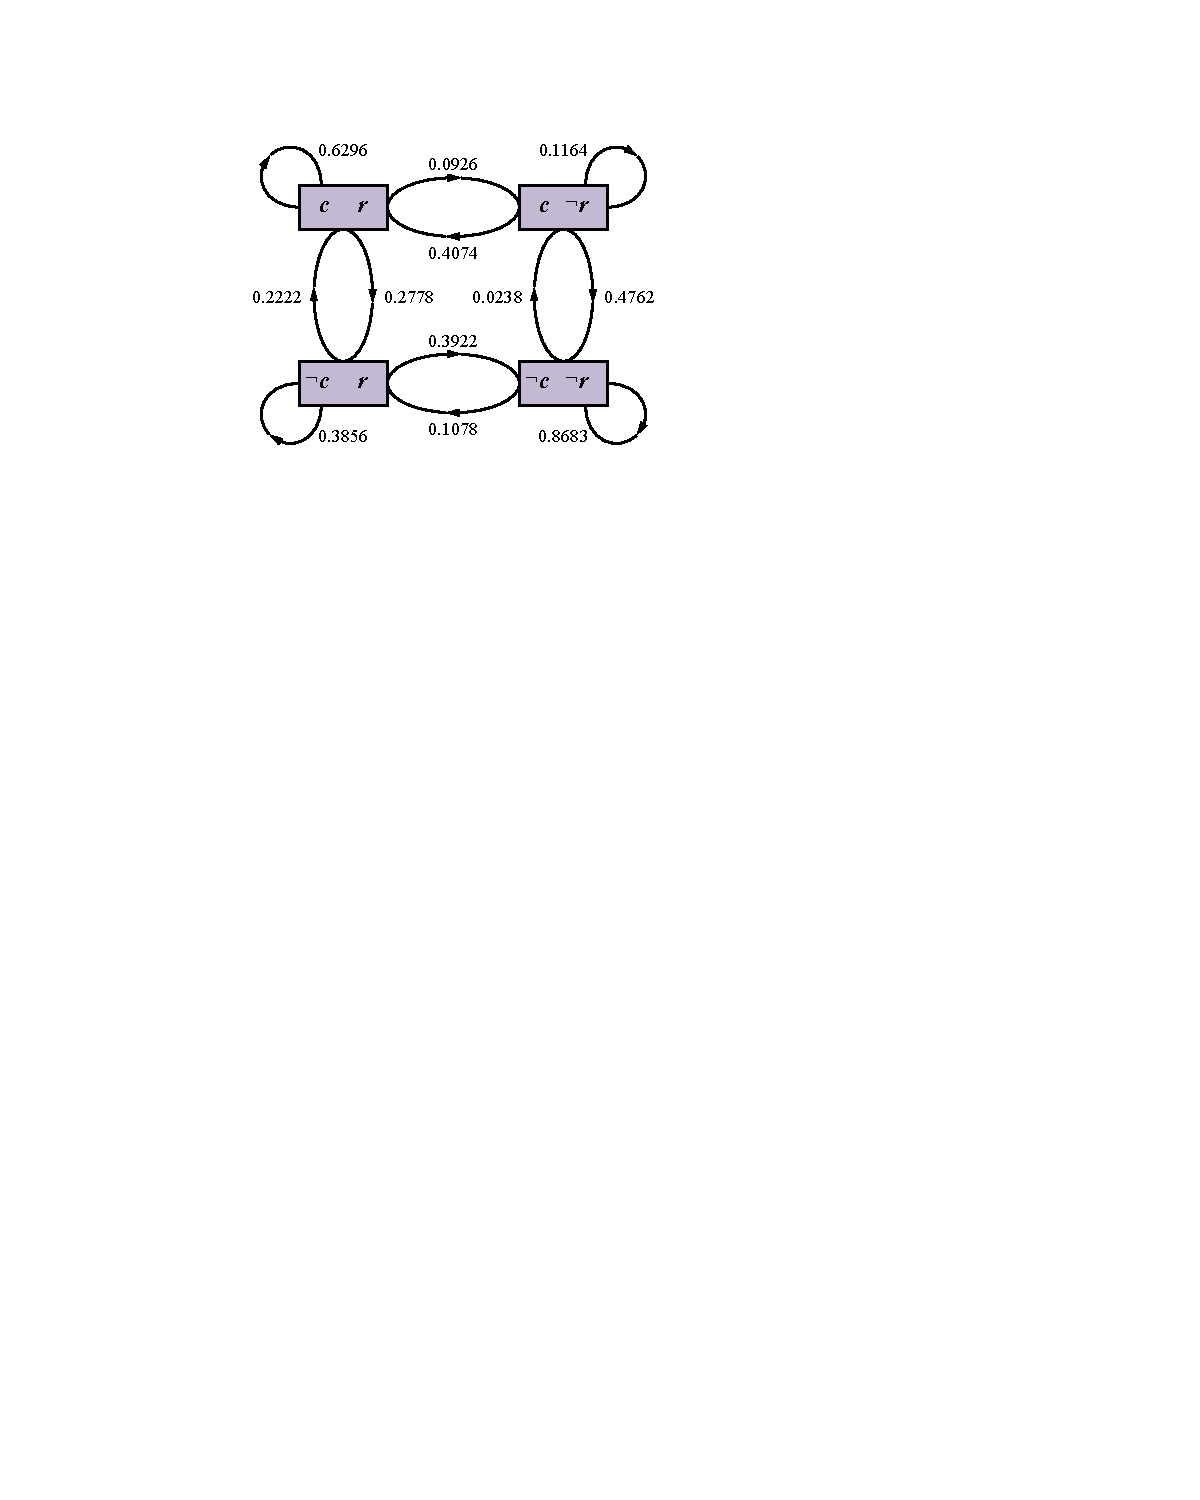
\includegraphics[alt={aima fig 13_21_a markov chain gibbs sampling example},width=0.75\linewidth]{aima-fig-13_21_a-markov-chain-gibbs-sampling-example.pdf}
\section{Gibbs Sampling Algorithm}
\label{sec:orgd82e429}


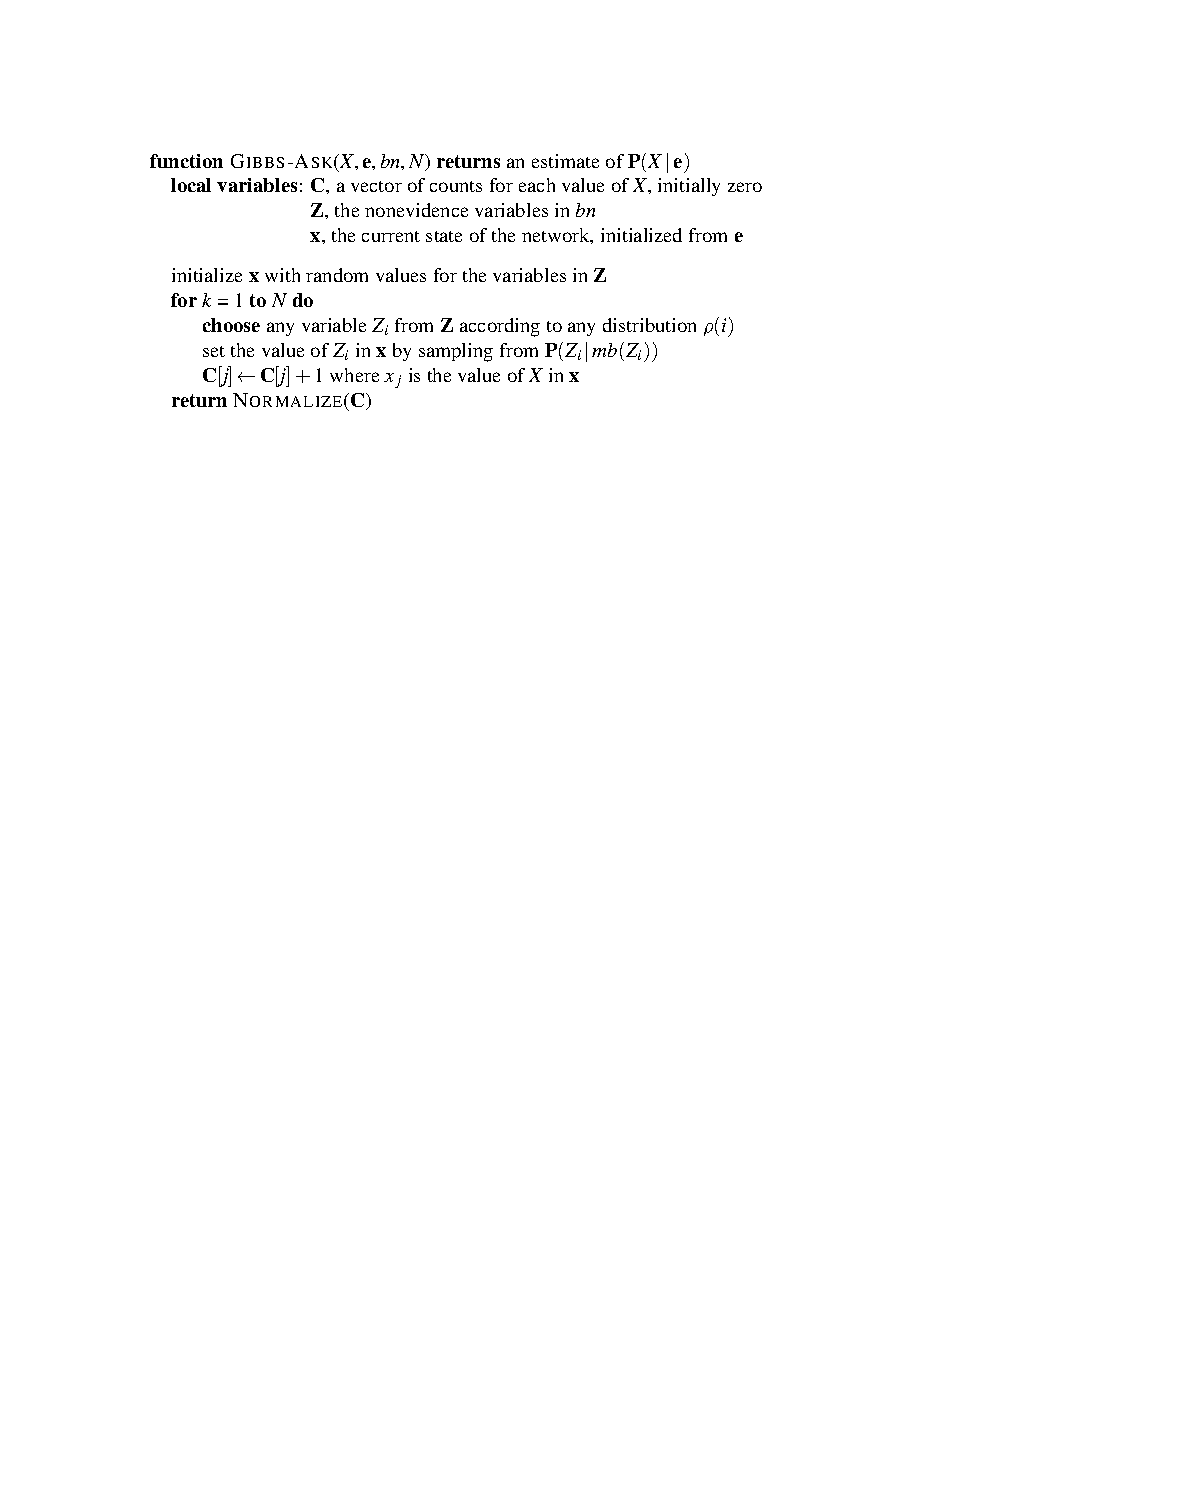
\includegraphics[alt={aima fig 13_20 bayes net gibbs sampling algorithm},width=0.75\linewidth]{aima-fig-13_20-bayes-net-gibbs-sampling-algorithm.pdf}
\section{Gibbs Sampling vs. Importance Sampling}
\label{sec:orgb919a0f}

Performance of Gibbs sampling compared to likelihood weighting on the car
insurance network.


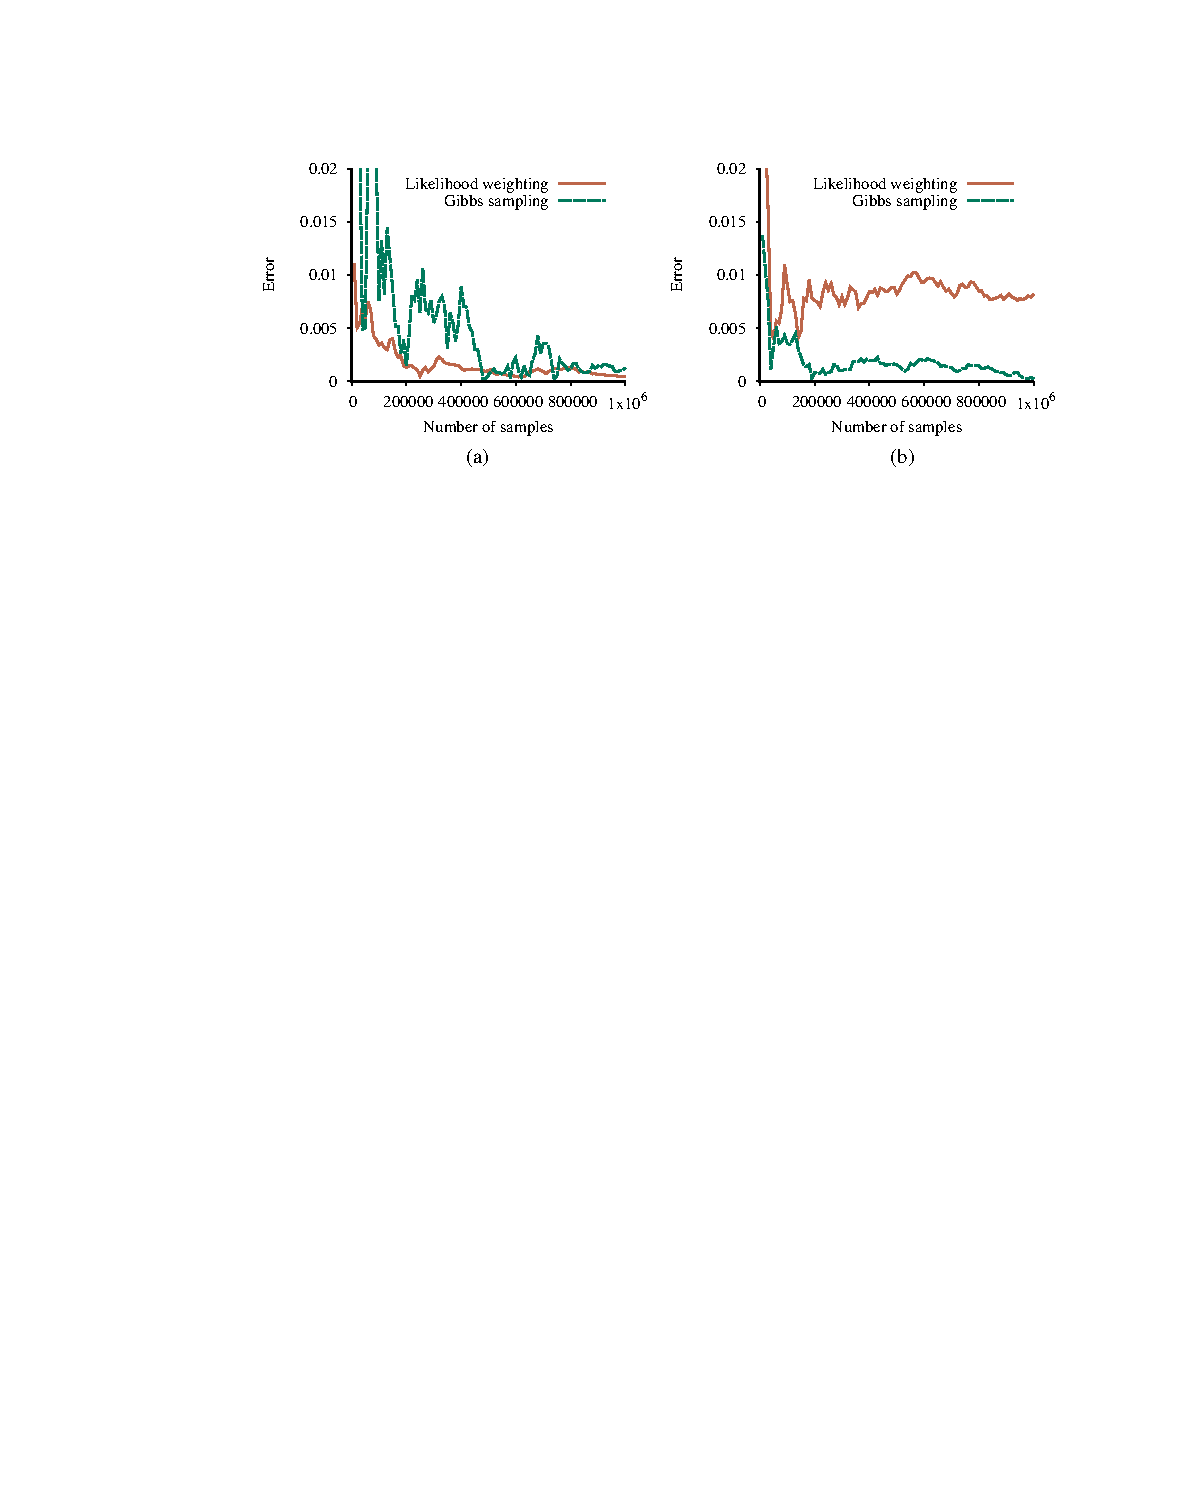
\includegraphics[alt={aima fig 13_22 performance plots gibbs sampling likelihood weighting},width=0.75\linewidth]{aima-fig-13_22-performance-plots-gibbs-sampling-likelihood-weighting.pdf}


\begin{itemize}
\item (a) for the standard query on \(PropertyCost\), and
\item (b) for the case where the output variables are observed and \(Age\) is the query variable.
\end{itemize}

Gibbs sampling typically outperforms likelihood weighting when evidence is mostly downstream.
\section{Markov Chains}
\label{sec:org0aef624}


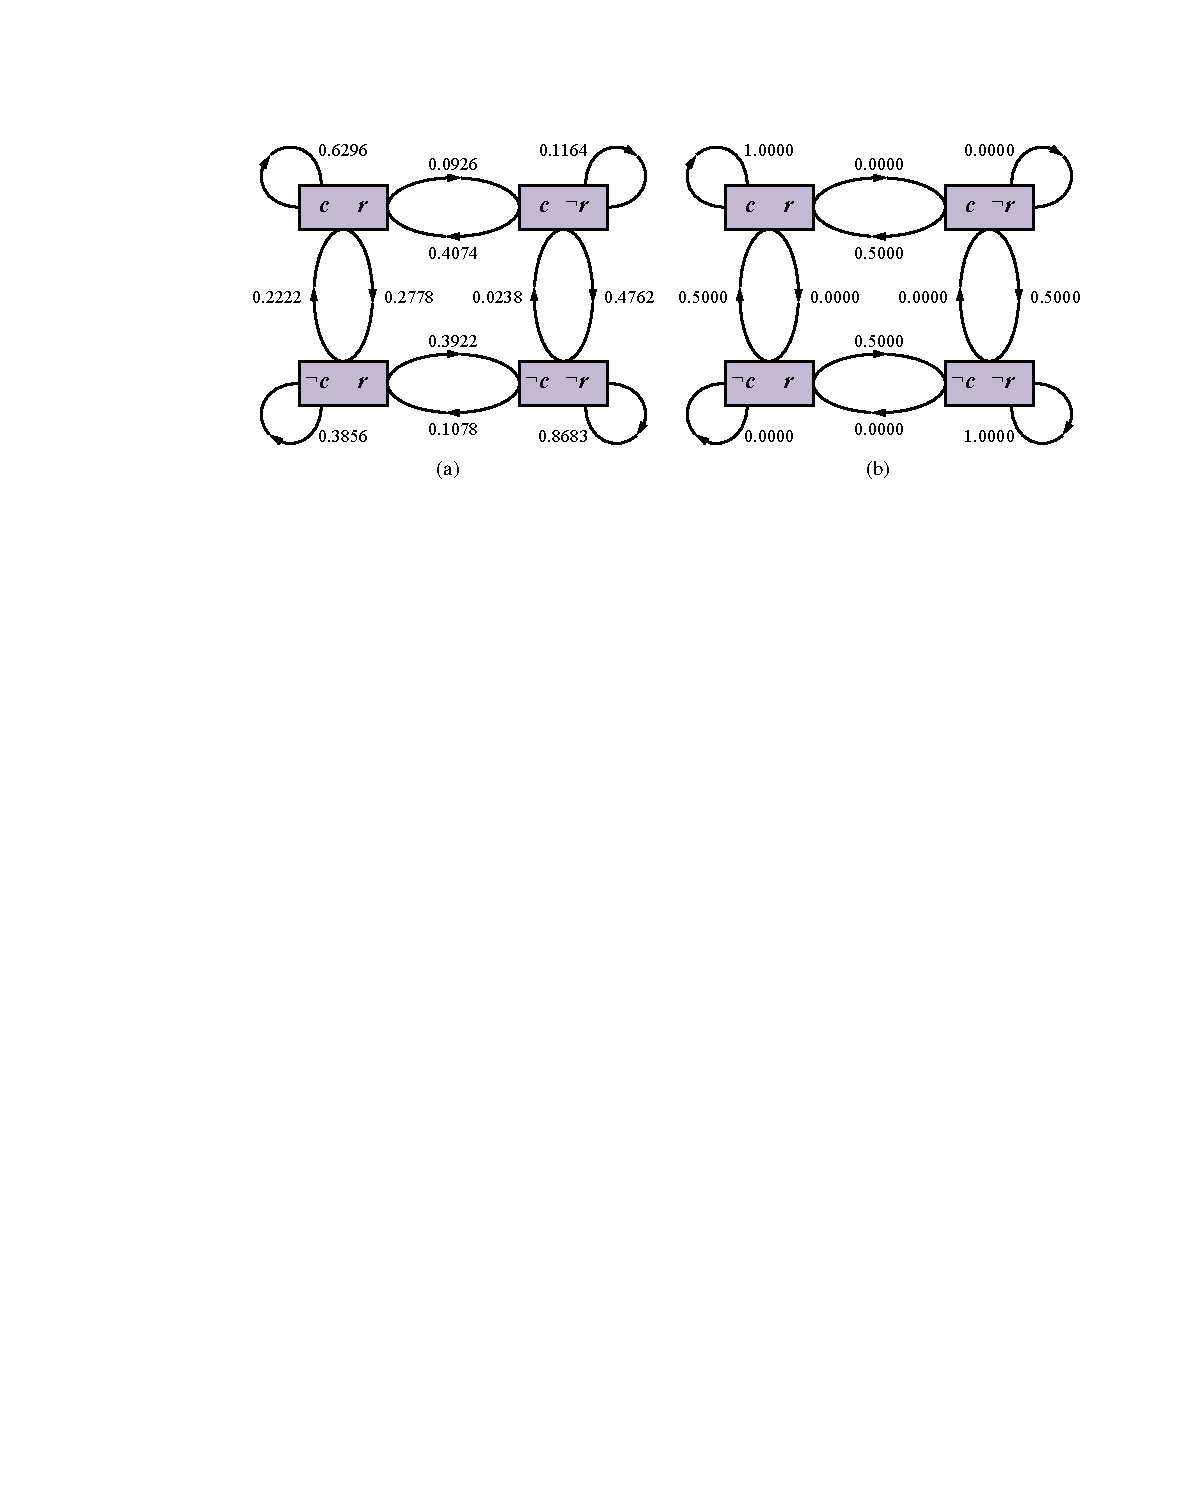
\includegraphics[alt={aima fig 13_21 markov chain},width=0.75\linewidth]{aima-fig-13_21-markov-chain.pdf}


\begin{itemize}
\item (a) The states and transition probabilities of the Markov chain for the query \(P(Rain|Sprinkler= true,WetGrass= true)\). Note the self-loops: the state stays the same when either variable is chosen and then resamples the same value it already has.

\item (b) The transition probabilities when the CPT for \(Rain\) constrains it to have the same value as \(Cloudy\).
\end{itemize}
\section{Metropolis}
\label{sec:orgc85cfdb}



\includegraphics[alt={metropolis},height=3.2in]{metropolis.jpg}
\section{Metropolis-Hastings Sampling}
\label{sec:org6ee8b42}

Like simulated annealing, MH has two stages in each iteration of the sampling process:

\begin{enumerate}
\item Sample a new state \(x'\) from a \textbf{proposal distribution} \(q(x'|x)\), given the current state \(x\).

\item Probabilistically accept or reject \(x'\) according to the \textbf{acceptance probability}
\end{enumerate}

\[
a(x'|x) = \min \left( 1, \frac{ \pi(x') q(x|x') } {\pi(x) q(x'|x)} \right)
\]

If the proposal is rejected, the state remains at \(x\).

\(q(x'|x)\) could be defined as follows:

\begin{itemize}
\item With probability 0.95, perform a Gibbs sampling step to generate \(x'\).

\item Otherwise, generate \(x'\) by running WEIGHTED-SAMPLE using likelihood weighting.
\end{itemize}

This has the effect of getting MH "unstuck."
\end{document}
